\documentclass[a4paper,12pt]{article}
\usepackage{a4wide}
\usepackage[pdftex]{hyperref}
\usepackage[german]{babel}
\usepackage[utf8]{inputenc}
\usepackage{amssymb}
\usepackage{csquotes}
\usepackage{wrapfig}
\usepackage{graphicx}
\usepackage{multicol}
\usepackage{amsmath}
\usepackage{enumitem}
\usepackage{polynom}
\usepackage{siunitx}

\setlength{\marginparsep}{1 cm}
\setlength{\topmargin}{-0.6in}
\setlength{\textheight}{9.5in}
\pagestyle{plain}

\polyset{%
   style=C,
   delims={\big(}{\big)},
   div=:
}

% Polynomial long division
\polyset{%
	style=C,
	delims={\big(}{\big)},
	div=:
}

% Differential operator
\newcommand{\diff}[1]{\:\mathrm{d}{#1}}
\newcommand{\pdd}[2]{\frac{\partial #1}{\partial #2}}
\newcommand{\pddn}[3]{\frac{\partial^{#1} #2}{\partial #3^{#1}}}
\newcommand{\dd}[2]{\frac{\mathrm{d}{#1}}{\mathrm{d}{#2}}}
\newcommand{\ddn}[3]{\frac{\mathrm{d}^{#1}{#2}}{\mathrm{d}{#3^{#1}}}}

% N-th root
% \nroot{3}{27}
\newcommand*{\nroot}[2]{\sqrt[\leftroot{-1}\uproot{2}#1]{#2}}
\newcommand*{\ncroot}[4]{\sqrt[\leftroot{#1}\uproot{#2}#3]{#4}}

% 2 component vector
% \tvect{1}{-1}
% \tvec{1}{-1}
\newcommand{\tvect}[2]{%
   \ensuremath{\Bigl(\negthinspace\begin{smallmatrix}#1\\#2\end{smallmatrix}\Bigr)}}
\newcommand{\tvec}[2]{%
    \ensuremath{\left(\negthinspace\begin{matrix}#1\\#2\end{matrix}\right)}}

% 3 component vector
% \rvect{1}{-1}{0}
% \rvec{1}{-1}{0}
\newcommand{\rvect}[3]{%
   \ensuremath{\Bigl(\negthinspace\begin{smallmatrix}#1\\#2\\#3\end{smallmatrix}\Bigr)}}
\newcommand{\rvec}[3]{%
    \ensuremath{\left(\negthinspace\begin{matrix}#1\\#2\\#3\end{matrix}\right)}}

% Long vector arrow
% \xshlongvec{ABC}

% German-style quotation marks %
\MakeOuterQuote{"}

% Number sets
\newcommand{\N}{\mathbb{N}}
\newcommand{\Z}{\mathbb{Z}}
\newcommand{\Q}{\mathbb{Q}}
\newcommand{\R}{\mathbb{R}}
\newcommand{\C}{\mathbb{C}}

\newcommand{\setzero}{\varnothing}

% Mention (small caps)
\newcommand{\mention}[1]{\textsc{#1}}

% Functions
\newcommand{\asin}[0]{\text{asin}}
\newcommand{\acos}[0]{\text{acos}}
\newcommand{\atan}[0]{\text{atan}}
\newcommand{\sgn}[0]{\text{sgn}}
\newcommand{\grad}[0]{\text{grad}}

% Scale
% Usage in math mode: \Scale[1.5]{...equation...} %
\newcommand*{\Scale}[2][4]{\scalebox{#1}{$#2$}}%

% Units
\newcommand{\um}{\text{m}}
\newcommand{\us}{\text{s}}
\newcommand{\ukm}{\text{km}}
\newcommand{\ukg}{\text{kg}}
\newcommand{\uh}{\text{h}}
\newcommand{\ukmh}{\frac{\ukm}{\uh}}
\newcommand{\umpers}{\frac{\um}{\us}}
\newcommand{\umss}{\frac{\ukm}{\us^2}}
\newcommand{\ukgss}{\frac{\ukg}{\us^2}}
\newcommand{\degrees}[1]{\SI{#1}{\degree}}

% Floor / ceil
\newcommand{\floor}[1]{\left\lfloor #1 \right\rfloor}
\newcommand{\ceil}[1]{\left\lceil #1 \right\rceil}

% Circle characters
\newcommand*\circled[1]{
    \tikz[baseline=(char.base)]{
        \node[shape=circle,draw,inner sep=2pt] (char) {#1};
    }
}



\begin{document}

\begin{center}
  {\bf {\large Aufgabenblatt 4 (MI/IT 2020)}}
\end{center}

% Tasks

\begin{enumerate}

\item Beweisen Sie, dass $\dd{}{x}\ln(x) = \frac{1}{x}$ gilt, in dem Sie von $f(x) = e^x$ ausgehen und die Regel zur Ableitung der Umkehrfunktion anwenden! ($\dd{y}{x}\cdot\dd{x}{y}=1$)

\item Zeigen Sie anhand der Definition von $\sinh(x)$ und $\cosh(x)$ über die Exponentialfunktion, dass die Beziehung $\cosh^2(x)-\sinh^2(x)=1$ gilt! Berechnen Sie damit die Ableitung von $\tanh(x) = \frac{\sinh(x)}{\cosh(x)}$!

\item
$f(u,v,w) = \frac{u^2 \sin(3v) +4}{w}$.
Leiten Sie f partiell nach u, nach v und nach w ab, d.h. bestimmen Sie $\frac{\partial^2 f}{\partial u \partial v}(u,v,w)$, $\frac{\partial^2 f}{\partial v \partial u}(u,v,w)$ sowie $\frac{\partial^2 f}{\partial w^2}(u,v,w)$! Stimmt bei diesem Beispiel der Satz von Schwarz?



\item{Bestimmen Sie die Fläche zwischen der Funktion $y=x^2-5x+6$ und der $x$-Achse im Intervall $[1;5]$, wobei die Flächen unterhalb der $x$-Achse positiv gezählt werden.}



\item Es soll das unbestimmte Integral der Funktion $f(x) = \frac{x^2+2}{x^3-4x}$ ermittelt werden. Führen Sie zuerst eine Partialbruchzerlegung durch und geben Sie dann das Integral an!


\item Berechnen Sie die Integrale $\int \sin^2(x) \diff{x}$ und $\int \cos^2(x) \diff{x}$ mittels einmaliger partieller Integration! (Hinweis: Trigonometrischer Pythagoras, nach dem gesuchten Integral umstellen.)

\item (*) Die Fakultät $a_z = (z-1)!$ einer natürlichen Zahl  $z$ ist charakterisiert durch die rekursive Eigenschaft $a_{z+1} = z\cdot a_z$. Für nichtganzzahlige Werte $z$ wird sie erweitert zu der sogennanten Gamma-Funktion, diese ist definiert als $\Gamma(z) = \int\limits_0^\infty x^{z-1} e^{-x} \d x$. Zeigen Sie mittels partieller Integration, dass auch die Gammafunktion diese rekursive Eigenschaft erfüllt, d.h. dass $\Gamma(z+1) = z \cdot \Gamma(z)$ gilt!


\item Sei $f$ eine integrierbare Funktion und $F$ deren Stammfunktion. Zeigen Sie durch Substitution, dass $\int f(mx+n) \diff{x} = \frac{1}{m} F(mx+n) + C$ gilt ($m,n\in\R$)! Was ergibt sich also für $\int (3x-5)^{100} \diff{x}$?

\item Gebietsintegral in kartesischen Koordinaten: Der Bereich $0 \le x \le \pi$ und $0 \le y \le \sin(x)$ ist mit der Masse der Dichte $\rho(x,y)=1+x+4y$ belegt. Skizzieren Sie diesen Bereich und berechnen Sie seine Gesamtmasse! (Hinweis: Die Masse ergibt sich durch Integration der Dichte über den Bereich.)

\item Gebietsintegral in Polarkoordinaten. Durch $0 \le a \le r \le b$ und $0 \le \varphi \le \frac{\pi}{2}$ ist ein Gebiet gegeben (Radius $r$, Winkel $\varphi$, $a,b\in\R$). Skizzieren Sie es für $a=1$, $b=2$! Berechnen Sie anschließend das Gebietsintegral von $f(x,y)=x\cdot y$ über diesen Bereich! (Hinweis: $x$ und $y$ zuerst durch Polarkoordinaten $r,\varphi$ ausdrücken.)


\item Gesucht sind die Extremstellen der Funktion $f(x,y) = 4(x-2)(y^2+10y)+3x^3$. Finden Sie anhand der notwendigen Bedingung Kandidaten für Extremstellen. Prüfen Sie anhand des Kriteriums $\Delta = f_{xx}\cdot f_{yy}-f_{xy}\cdot f_{yx} > 0$, ob es sich wirklich um Extremstellen handelt. Falls ja, handelt es sich um Minima oder Maxima?


\end{enumerate}

\newpage

% Solutions

\begin{center}
{\bf {\large Lösungen}}
\end{center}

\begin{enumerate}
	
\item Es ist $y=e^x$ und $\dd{y}{x} = e^x$. Die Regel zur Ableitung der Umkehrfunktion liefert:

\begin{alignat*}{1}
	e^x  \cdot \dd{x}{y} &= 1 \\
	\dd{x}{y} &= \frac{1}{e^x} \\
	\dd{x}{y} &= \frac{1}{y}
\end{alignat*}

Im letzten Schritt benutzt, dass $y=e^x$ ist. Da aus $y=e^x$ durch Umstellen $x=\ln(y)$ folgt und wie eben gezeigt $\dd{x}{y} = \frac{1}{y}$ gilt, haben wir die Aussage bewiesen.

\item Wir setzen die Definition für den Hyperbelkosinus und Hyperbelsinus ein und vereinfachen:

\begin{alignat*}{1}
	\cosh^2(x)-\sinh^2(x) &= \left(\frac{e^x+e^{-x}}{2}\right)^2 + \left(\frac{e^x-e^{-x}}{2}\right)^2 \\
	                      &= \frac{\left(e^x+e^{-x}\right)^2 - \left(e^x-e^{-x}\right)^2}{4} \\
	                      &= \frac{\left(e^{2x}+e^{-2x}+2e^xe^{-x}\right) - \left(e^{2x}+e^{-2x}-2e^xe^{-x}\right)}{4} \\
	                      &= \frac{2+2}{4} \\
	                      &= 1
\end{alignat*}

Wobei wir $e^xe^{-x} = e^0 = 1$ benutzt haben.

Für die Ableitung des Hyperbeltangens $\tanh$ folgt damit analog zur Ableitung des Tangens über die Produkt- beziehungsweise Quotientenregel:

\begin{alignat*}{1}
	\dd{}{x} \tanh(x) &= \dd{}{x} \frac{\sinh(x)}{\cosh(x)} \\
	                  &= \frac{\cosh^2(x)-\sinh^2(x)}{\cosh^2(x)} \\
	                  &= \frac{1}{\cosh^2(x)}
\end{alignat*}

Alternativ hätten wir im letzten Schritt auch vereinfachen können:

$$
	\dd{}{x} \tanh(x) = 1 - \frac{\sinh^2(x)}{\cosh^2(x)} = 1-\tanh^2(x)
$$


\item

$\frac{\partial f}{\partial u} = \frac{2u\sin(3v)}{w}$

$\frac{\partial f}{\partial v} = \frac{3u^2\cos(3v)}{w}$

$\frac{\partial^2 f}{\partial u \partial v} = \frac{\partial^2 f}{\partial v \partial u} = \frac{6u \cos(3v)}{w}$

$\frac{\partial^2 f}{\partial w^2} = (u^2\sin(3v)+4)\cdot \frac{2}{w^3}$

Bei richtiger Rechnung ergibt sich $\frac{\partial^2 f}{\partial u \partial v} = \frac{\partial^2 f}{\partial v \partial u}$, es liegt also kein Widerspruch zum Satz von Schwarz vor. 


	
\item

Zuerst müssen wir wissen, wo die Funktion unterhalb bzw. oberhalb der x-Achse liegt. Dazu berechnen wir die Nullstellen $f(x) = x^2-5x+6 = 0$ mittels p-q-Formel:

$$x_1 = 2, x_2 = 3$$

Also müssen wir die Flächen im Bereich $[1,2]$, $[2,3]$ und $[3,5]$ separat berechnen und die Werte anschließend betragsmäßig aufaddieren:

$$A = | \int\limits_1^2 f(x) \diff{x} | + | \int\limits_2^3 f(x) \diff{x} | + | \int\limits_3^5 f(x) \diff{x} | $$

Das unbestimmte Integral von $f$ lautet

$${\int f(x) \diff{x}} = \frac{1}{3} x^3 - \frac{5}{2} x^2 + 6x + C$$

Für den Flächeninhalt erhalten wir damit den Wert $A=5\frac{2}{3} = \frac{17}{3}$.



\item Der Nenner $x^3-4x$ besitzt die Nullstellen $-2, 0, 2$. Damit kann eine Partialbruchzerlegung angesetzt werden:

$$\frac{x^2+2}{x^3-4x} = \frac{A_1}{x-2} + \frac{A_2}{x} + \frac{A_3}{x+2}$$

Es ergibt sich $A_1$ = $\frac{3}{4}$, $A_2=-\frac{1}{2}$, und $A_3 = \frac{3}{4}$.

Damit lässt sich das Integral sofort angeben (Betragsstriche nicht vergessen!)

$$ \int f(x)\diff{x} = \frac{3}{4} \ln(|x-2|) - \frac{1}{2} \ln(|x|) + \frac{3}{4}\ln(|x+2|)$$


\item Wir wenden zuerst einmal partielle Integration an

$$
	\int \sin(x) \sin(x) \diff{x} = -\cos(x)\sin(x) + \int \cos^2(x) \diff{x}
$$

Als nächstes nutzen wir die trigonometrische Identität $\sin^2(x)+\cos^2(x)=1$ in der Form $\cos^2(x) = 1-\sin^2(x)$:

\begin{alignat*}{1}
	\int \sin^2(x) \diff{x} &= -\cos(x)\sin(x) + \int 1-\sin^2(x) \diff{x} \\
	                        &= -\cos(x)\sin(x) + x - \int \sin^2(x) \diff{x}
\end{alignat*}

Auf der linken und rechten Seite der Gleichung steht das zu bestimmende Integral $\int \sin^2(x)\diff{x}$. Wenn wir nach diesem umstellen, erhalten wir:

\begin{alignat*}{1}
	\int \sin^2(x) \diff{x} = \frac{1}{2} (x-\cos(x)\sin(x))
\end{alignat*}

Analog können wir vorgehen, um $\int \cos^2(x) \diff{x}$ zu berechnen. Eine weitere Möglichkeit besteht darin, dass oben in der ersten Gleichung ein Zusammenhang zwischen dem Integral von $\cos^2(x)$ und $\sin^2(x)$ hergestellt wird. Wenn wir diese Gleichung umstellen, erhalten wir:

$$
	\int \sin^2(x) \diff{x} + \cos(x)\sin(x) = \int \cos^2(x) \diff{x}
$$

Da Integral über $\sin^2(x)$ kennen wir bereits und erhalten:

$$
	\int \cos^2(x) \diff{x} =  \frac{1}{2} (x-\cos(x)\sin(x)) + \cos(x)\sin(x) = \frac{1}{2} (x+\cos(x)\sin(x))
$$

\item $\Gamma(z+1) = \int_0^\infty x^z e^{-x} \diff{x}$ \\
 $= \underbrace{\big[ -x^z e^{-x}\big]_{0}^{\infty}}_{=0-0} + z \underbrace{\int_0^\infty x^{z-1}e^{-x}\diff{x}}_{\Gamma(z)} = z\cdot\Gamma(z)$



\item Wir substituieren $z=mx+n$. Es ist $z'(x)=mx$, also $\diff{x} = \diff{z}/m$. Eingesetzt in das Integral folgt:

\begin{alignat*}{1}
	\int f(mx+n) \diff{x} &= \int f(z) \frac{\diff{z}}{m} \\
	                      &= \frac{1}{m} \int f(z) \diff{z} \\
	                      &= \frac{1}{m} F(z) + C\\
	                      &= \frac{1}{m} f(mx+n) + C
\end{alignat*}

Dies war zu zeigen. Obige Regel nennt man auch lineare Substitution und ermöglicht, das Integral von verschobenen und skalierten Funktion einfach zu berechnen. Beispielsweise folgt damit sofort $\int (3x-5)^{100} \diff{x} = \frac{1}{3\cdot 101} (3x-5)^{101} + C$

\item Die $x$-Werte laufen im von $0$ bis $\pi$. Die $y$-Werte fangen immer bei $0$ an und hören abhängig vom $x$-Wert bei $\sin(x)$ auf. Der Bereich ist also gegeben durch den ersten Bauch der Sinus-Funktion, siehe Abbildung \ref{fig:Area}.

Wir integrieren also zuerst über $y$ und anschließend über $x$, um die Masse $M$ zu berechnen:

\begin{alignat*}{1}
	M  &= \int\limits_0^\pi \left( \int_0^{\sin(x)} 1+x+4y \diff{y} \right) \diff{x} \\
	   &= \int\limits_0^\pi \left( \left[ y + xy + 2y^2 \right]\Biggr|_{y=0}^{y=\sin(x)} \right) \diff{x} \\
	   &= \int\limits_0^\pi  \sin(x)+x\sin(x)+2\sin^2(x) \diff{x} \\
	   &= [-\cos(x)]\Biggr|_{0}^{\pi} + [\sin(x)-x\cos(x)]\Biggr|_{0}^{\pi} + [x-\cos(x)\sin(x)]\Biggr|_{0}^{\pi} \\
	   &= 1 - (-1) + \pi + \pi \\
	   &= 2 + 2\pi
\end{alignat*}

\begin{figure}
	\centering
	\includegraphics[width=0.8\textwidth]{../gnuplot/ex-area-integral-img-a}
	\caption{Gebiet $0 \le x \le \pi$ und $0 \le y \le \sin(x)$}
	\label{fig:Area}
\end{figure}


\item Bei dem Gebiet handelt es sich um einen Kreisring mit Innenradius $1$ und Außenradius $2$, welcher von $\degrees{0}$ bis $\degrees{45}$ läuft. Über geometrische Beziehungen am Kreis erhält man $x=r\cos(\varphi)$ und $y=r\sin(\varphi)$. Somit müssen wir berechnen:

\begin{alignat*}{1}
	  & \int\limits_a^b \left( \int\limits_0^{\pi/2} r \cdot r^2 \sin(\varphi)\cos(\varphi) \diff{\varphi} \right) \diff{r} \\
	= & \int\limits_a^b r^3 \left( \int\limits_0^{\pi/2} \sin(\varphi)\cos(\varphi) \diff{\varphi} \right) \diff{r} \\
	= & \int\limits_a^b r^3 \left( \frac{1}{2}\sin^2(x) \right) \Biggr|_{0}^{\pi/2} \diff{r} \\
	= & \int\limits_a^b \frac{1}{2} r^3  \diff{r} \\
	= & \frac{1}{2} \cdot \frac{r^4}{4}\Biggr|_a^b \\
	= & \frac{1}{8} (b^4-a^4)
\end{alignat*}


\item

Wir berechnen zuerst Kandidaten für die Extrempunkte. Die Ableitungen lauten:

$f_x(x,y) = 4(y^2+10y)+9x^2$

$f_y(x,y) = 4(x-2)(2y+10)$

Aus $f_y = 0$ folgt $x=2 \lor y=-5$.

\begin{enumerate}
\item $x=2$

Wir setzen  $x=2$ in $f_x(x,y) = 0$ ein:

$f_x(2,y) = 0 = 4y^2+40y+36$

$\implies y = -5 \pm \sqrt{25-9}$

$\implies y = -9 \lor y = -1$

\item $y=-5$

$f_x(x,-5) = 0 = 4 \cdot (25-50)+9x^2 = -100+9x^2$

$\implies x^2 = \frac{100}{9}$

$\implies x=-\frac{10}{3} \lor x=\frac{10}{3}$

\end{enumerate}

Wir erhalten also die 4 möglichen Stellen $(2|-1), (2|-9), (\frac{10}{3}|-5)$ und $(-\frac{10}{3}|-5)$.

Zum Überprüfen, ob es sich um Minima, Maxima oder Sattelpunkte handelt, benötigen wir noch die 2. Ableitungen:

$f_{xy}(x,y) = 8(y+5)$

$f_{xx}(x,y) = 18x$

$f_{yy}(x,y) = 8(x-2)$

Wir erhalten damit für die 4 Stellen:

\begin{enumerate}
\item $(2|-1)$: $f_{xx}=36, f_{yy}=0, f_{xy}=32, \Delta = -1024$
\item $(2|-9)$: $f_{xx}=36, f_{yy}=0, f_{xy}=-32, \Delta = -1024$
\item $(\frac{10}{3}|-5)$: $f_{xx}=60, f_{yy}=\frac{32}{3}, f_{xy}=0, \Delta = 640$
\item $(-\frac{10}{3}|-5)$: $f_{xx}=-60, f_{yy}=-\frac{128}{3}, f_{xy}=0, \Delta = 2560$
\end{enumerate}

Somit sind bei $(2|-1)$ und $(2|-9)$ Sattelstellen (da $\Delta < 0$).

Bei $(\frac{10}{3}|-5)$ ist ein Minima (da $\Delta > 0$ und $f_{xx} > 0$) und bei $(-\frac{10}{3}|-5)$ ein Maxima (da $\Delta > 0$ und $f_{xx} < 0$).

\begin{figure}[ht]
  \centering
  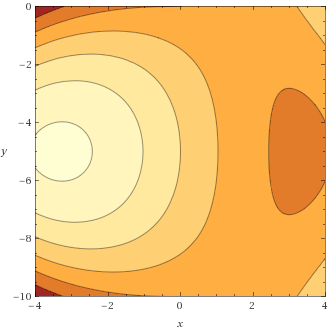
\includegraphics[width=0.8\textwidth]{../pool/ex-fn-extrema-6-img-c.png}
  \caption{Konturplot von $f(x,y) = 4(x-2)(y^2+10y)+3x^3$. Man erkennt die beiden Extremstellen. (dunkel: niedrige Funktionswerte, hell: große Frunktionswerte)}
  \label{ex-fn-extrema-6-img-c}
\end{figure}

\begin{figure}[ht]
  \centering
  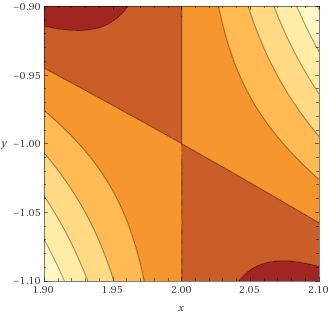
\includegraphics[width=0.8\textwidth]{../pool/ex-fn-extrema-6-img-d.png}
  \caption{Konturplot von $f(x,y) = 4(x-2)(y^2+10y)+3x^3$. Man erkennt eine Sattelstelle. (dunkel: niedrige Funktionswerte, hell: große Frunktionswerte)}
  \label{ex-fn-extrema-6-img-d}
\end{figure}

\begin{figure}[ht]
  \centering
  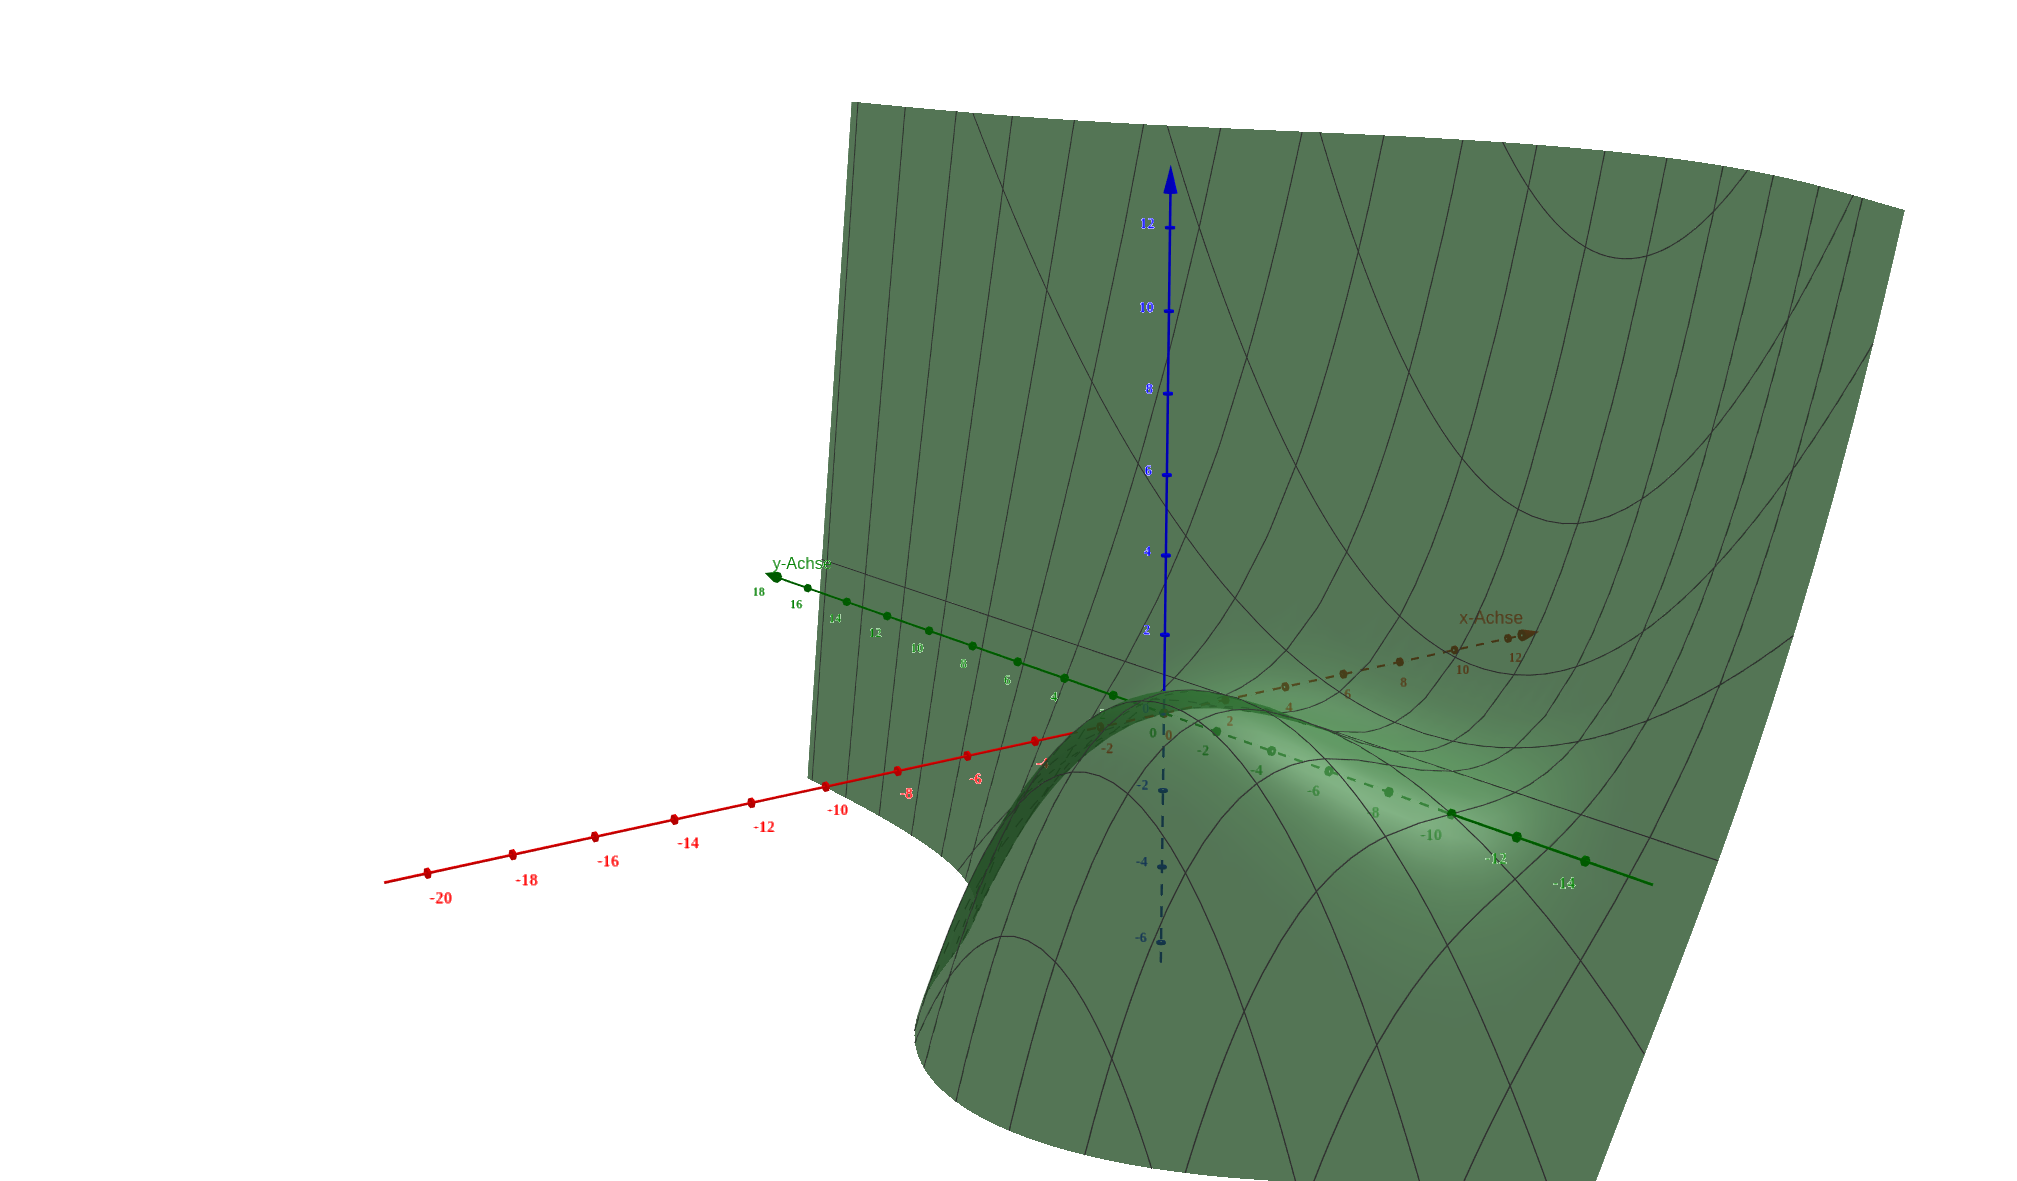
\includegraphics[width=0.8\textwidth]{../pool/ex-fn-extrema-6-img-a.png}
  \caption{3D-Plot von $f(x,y) = 4(x-2)(y^2+10y)+3x^3$}
  \label{ex-fn-extrema-6-img-a}
\end{figure}

\begin{figure}[ht]
  \centering
  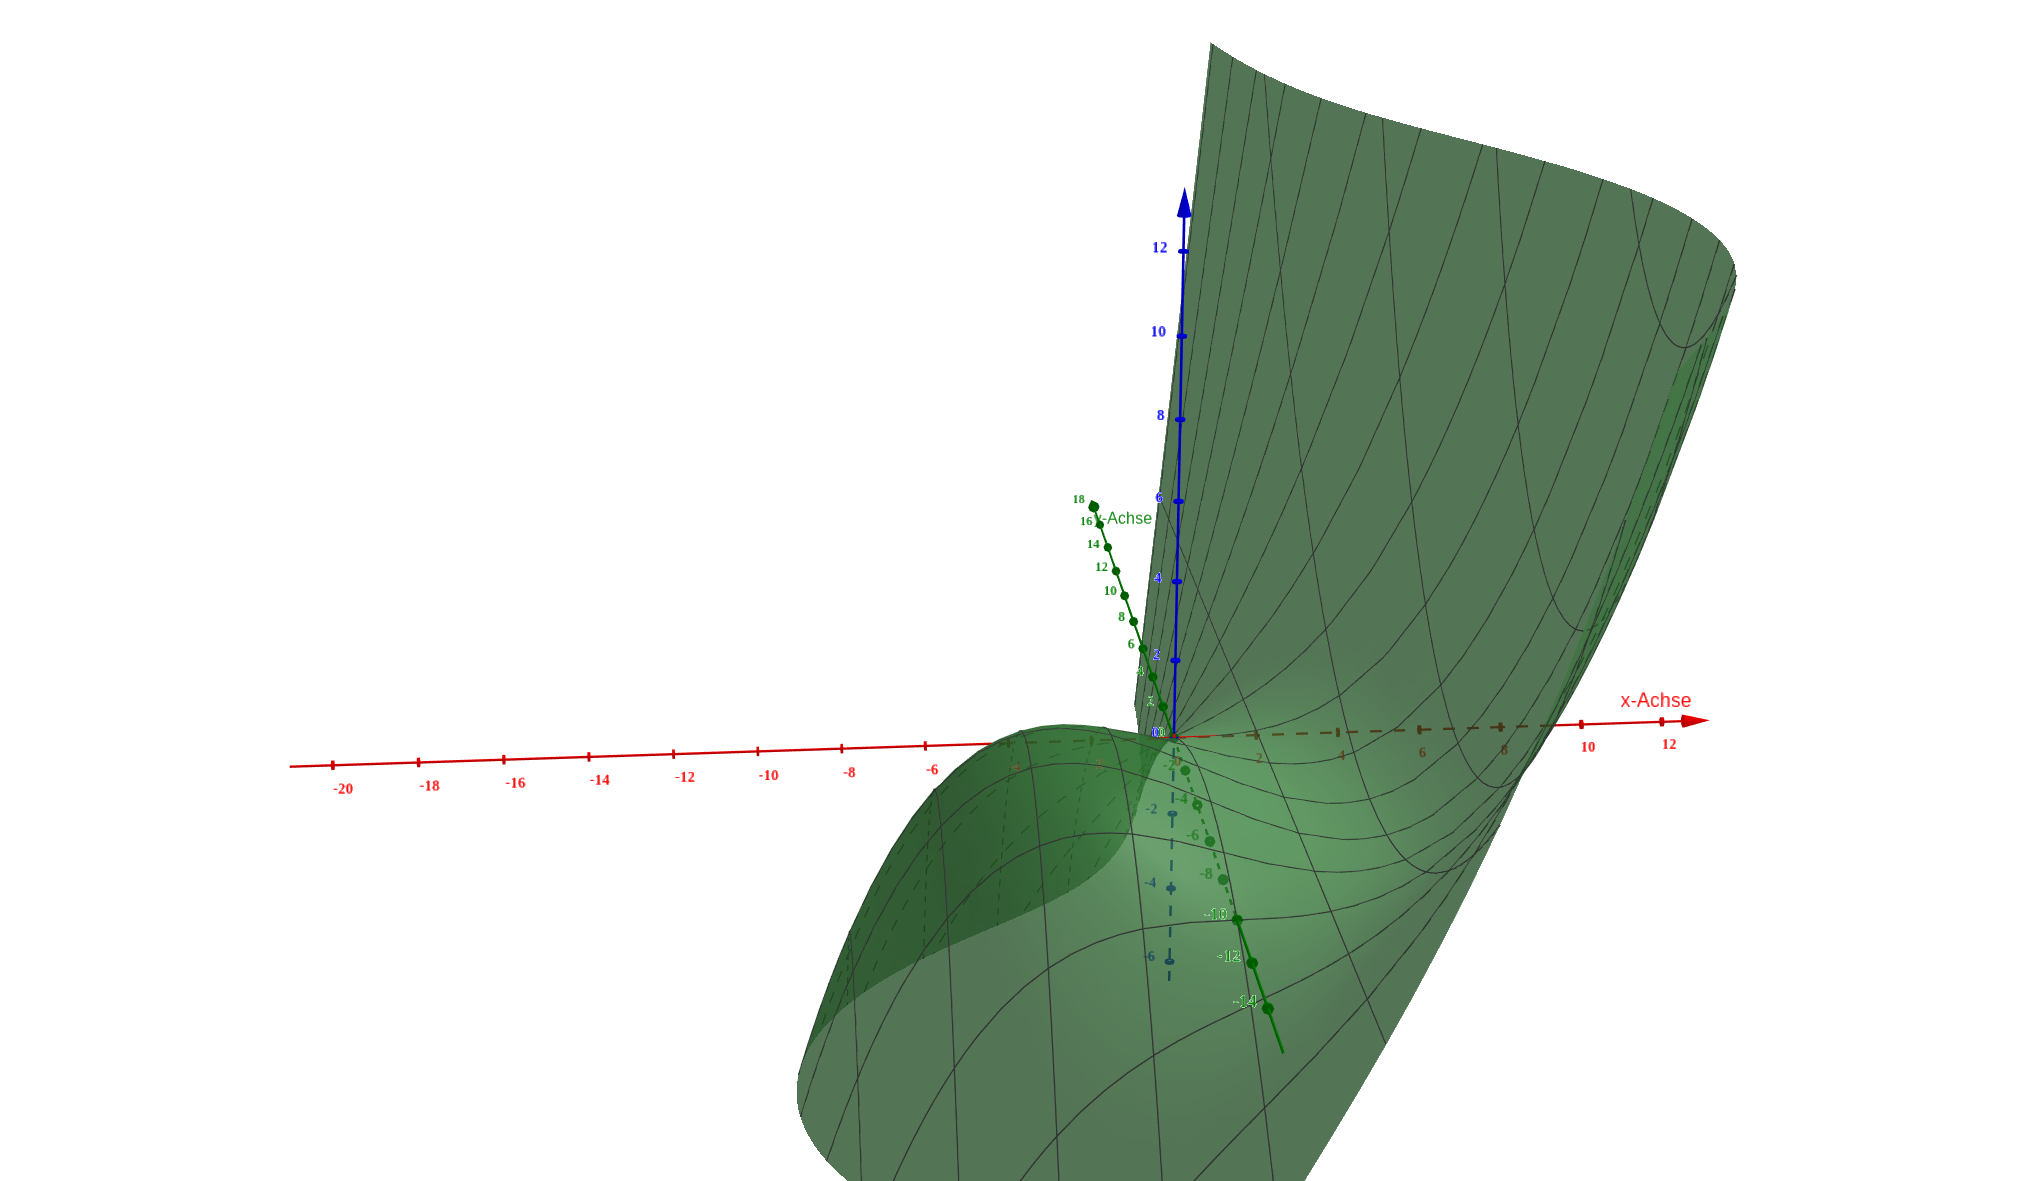
\includegraphics[width=0.8\textwidth]{../pool/ex-fn-extrema-6-img-b.png}
  \caption{3D-Plot von $f(x,y) = 4(x-2)(y^2+10y)+3x^3$}
  \label{ex-fn-extrema-6-img-b}
\end{figure}



\end{enumerate}

\end{document}

